\subsection{Configure Data Sources}
\label{sec:ui_configure_data_sources}

This dialog allows management of data sources, as stored in the configuration as well as in the database. \\

\begin{figure}[H]
    \hspace*{-2.5cm}
    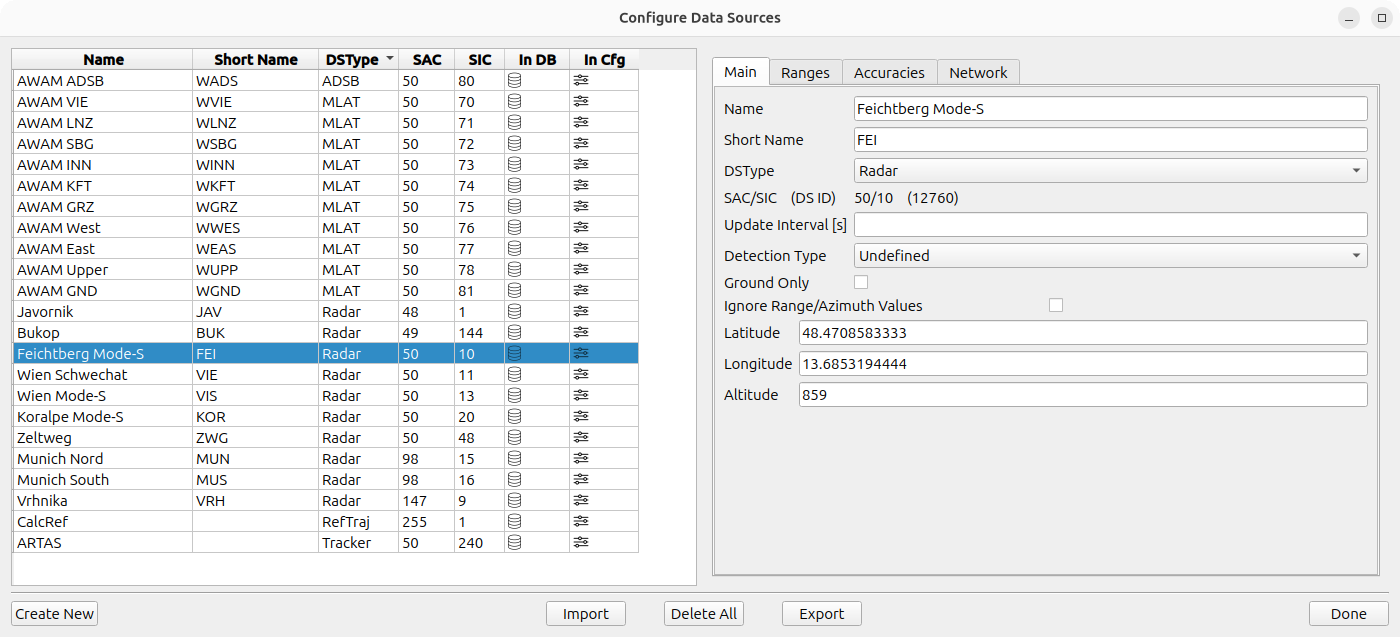
\includegraphics[width=19cm,frame]{figures/configure_data_sources.png}
  \caption{Configure Data Sources}
\end{figure}

If data is imported from ASTERIX, data source information might be missing, so this information must either be edited manually, or loaded from a previous configuration (or a previous database containing the same information). \\

A data source is always stored in the configuration, which means it is persistent and can be used in all new databases. 
It is useful to define all existing data sources in the configuration, since they are immediately used during import of data. \\

A data source is stored in the database only if data from said source is imported. 
During the import, if a data source can be found (matching SAC/SIC) in the configuration, it is automatically added to the database. \\

Please \textbf{note} that currently the position of data sources is only required for \textbf{Radar} data sources (in the plot position calculation), for all other data sources it would suffice to have SAC/SIC and name information for display purposes. \\

However, for CAT010, CAT020 and CAT062 the option exists to project from a Cartesian X/Y coordinate system to WGS84 latitude and longitude (when not available in the ASTERIX data). To use this feature during ASTERIX import, set a latitude/longitude for the respective data source.
\\

\paragraph {Data Sources Table Content}

\begin{itemize}
\item Name: Name of the data source
\item Short Name: Short name of the data source (optional)
\item DSType: Data source type, e.g. Radar, MLAT, ADS-B, ...
\item SAC: System Area Code, number between [0,255]
\item SIC: System Identification Code, number between [0,255]
\item DS ID: ID derived from SAC/SIC (255*SAC+SIC)
\item In DB: Indicator whether the data source is stored in the database
\item In Config: Indicator whether the data source is stored in the configuration
\end{itemize}
\ \\

When a data source is selected in the table, additional details are shown in the right side, where editing is also possible. \\

Please \textbf{note} that all changes to a data source are always written to the database as well as the configuration. \\

There are several tabs present:
\begin{itemize}
\item Main: Main information
\item Network: Optional network line information
\item For Radars
\begin{itemize}
\item Ranges: Optional detection ranges
\item Accuracy: Optional accuracy information
\end{itemize}
\item For MLAT
\begin{itemize}
\item MLAT Remote Units: Optional RU definition, for contributing receivers analysis
\end{itemize}
\end{itemize}
\ \\

\subsubsection {Main Tab}
Depending on the DSType, additional information can be set in a source. For all sources, the following information is given:

\begin{itemize}
\item Name: Name of the data source
\item Short Name: Short name of the data source (optional)
\item DSType: Data source type, e.g. Radar, MLAT, ADS-B, ...
\item SAC/SIC (DS ID): System Area Code, System Identification Code, derived data source ID
\item Detection Type: See below
\item Update Interval: Update interval in seconds (for correct labeling)
\item Ground Only: Check if the data source \textbf{only} provides detection for on-ground targets (e.g. for SMRs, local MLAT)
\end{itemize}
\ \\

For sources of DSType 'Radar', the following additional information should be provided:

\begin{itemize}
\item Latitude: Source center position as WGS-84 latitude, as floating point number in degrees, e.g. 42.0001
\item Longitude: Source center position as WGS-84 longitude, as floating point number in degrees, e.g. 17.01
\item Altitude: Source center altitude above MSL, in meters
\end{itemize}
\ \\

Additional optional information can be provided:

\begin{itemize}
\item Ignore Range/Azimuth values: Ignore such position information (if provided erroneously)
\end{itemize}
\ \\

\paragraph{Detection Type}

A detection type can be given for any data source, 'Unknown' is given as default. Currently only 'Primary Only' is used during reconstruction, but it is very important to set this type for SMRs, to mitigate sub-optimal association of primary-only target reports in close distances to clutter. \\

\begin{figure}[H]
  \center
    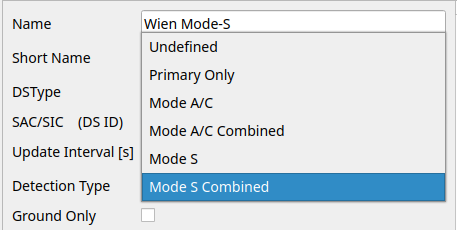
\includegraphics[width=8cm,frame]{figures/configure_ds_dettyp.png}
  \caption{Configure Data Sources: Detection Type}
\end{figure}

For primary-only data sources, additional JPDA settings for the reconstructor can be given:

\begin{itemize}
\item JPDA PD [1]: Probability of Detection, e.g. 0.9 for 90\%
\item Clutter Rate [1]: Rate of clutter detections per update interval, e.g. 10\\ in the given PSR Maximum range (has to be set below to take effect)
\end{itemize}
\ \\

\begin{figure}[H]
  \center
    \includegraphics[width=8cm,frame]{figures/configure_ds_jpda.png}
  \caption{Configure Data Sources: JPDA}
\end{figure}

\subsubsection {Network Tab}

\begin{figure}[H]
  \center
    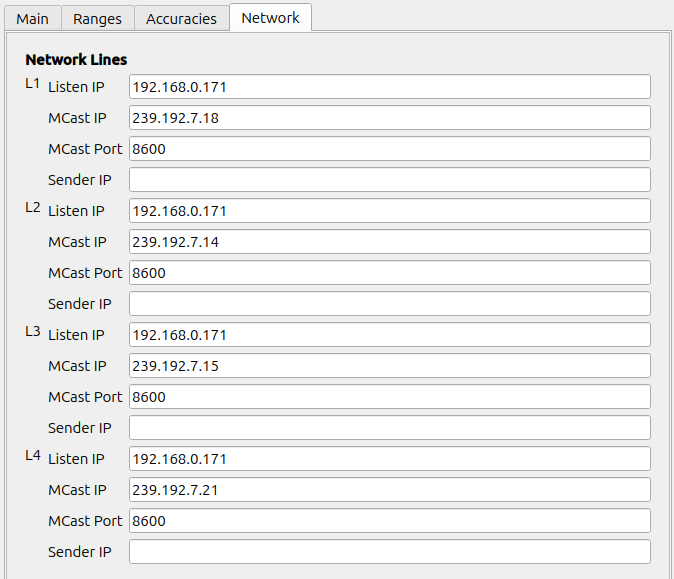
\includegraphics[width=8cm,frame]{figures/configure_network.png}
  \caption{Configure Data Sources: Network details}
\end{figure}

\begin{itemize}
\item 4 different lines are possible, each with 
\begin{itemize}
  \item Listen IP (defines used network interface and IGMP requests)
  \item Multicast IP
  \item Multicast port
  \item Sender IP (optional, for filtering purposes)
\end{itemize}
\end{itemize}
\ \\

Please note that for using real multicast addresses (inside of 224.0.0.0 to 239.255.255.255), it is recommended to also define the Listen IP to the local address of the network interface to be used. Otherwise the multicast data might not be received, or the wrong network interface might be used, causing COMPASS to receive no data. \\

Please note that if e.g. only Multicast IP and port are set, and the Multicast IP is set to a non-multicast one (outside of 224.0.0.0 to 239.255.255.255), a local replay is possible (without real multi-casting). \\

\subsubsection{Radar Ranges}

\begin{figure}[H]
  \center
    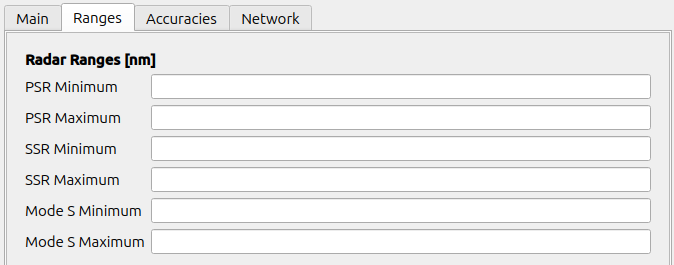
\includegraphics[width=8cm,frame]{figures/configure_radar_ranges.png}
  \caption{Configure Data Sources: Radar Ranges}
\end{figure}

\begin{itemize}
\item PSR Minimum: PSR minimum range, in nautical miles
\item PSR Maximum: PSR maximum range, in nautical miles
\item SSR Minimum: SSR minimum range, in nautical miles
\item SSR Maximum: SSR maximum range, in nautical miles
\item Mode S Minimum: Mode S minimum range, in nautical miles
\item Mode S Maximum: Mode S maximum range, in nautical miles
\end{itemize}

\subsubsection{Radar Accuracies}

\begin{figure}[H]
  \center
    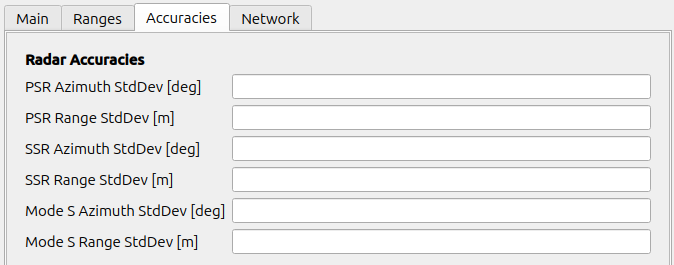
\includegraphics[width=8cm,frame]{figures/configure_radar_accuracies.png}
  \caption{Configure Data Sources: Radar Accuracies}
\end{figure}

\begin{itemize}
\item PSR Azimuth StdDev: PSR azimuth standard deviation, in degrees
\item PSR Range StdDev: PSR range standard deviation, in meters
\item SSR Azimuth StdDev: SSR azimuth standard deviation, in degrees
\item SSR Range StdDev: SSR range standard deviation, in meters
\item Mode S Azimuth StdDev: Mode S Radar azimuth standard deviation, in degrees
\item Mode S Range StdDev: Mode S Radar range standard deviation, in meters
\end{itemize}

\subsubsection{MLAT Remote Units}
\label{sec:ui_configure_ds_mlat_rus}

\begin{figure}[H]
  \center
    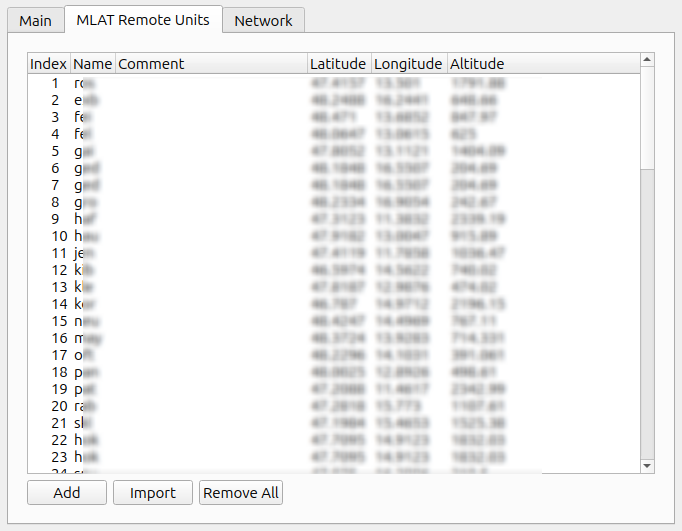
\includegraphics[width=12cm,frame]{figures/configure_mlat_rus.png}
  \caption{Configure Data Sources: MLAT Remote Units}
\end{figure}

For each MLAT data source, a list of remote units can be defined. Using such definitions, the contributing receivers information can be analyzed in the Table View or Geographic View. \\

For each remote unit, the following information can be provided:
\begin{itemize}
\item Index: Number of the RU, starting with 1 (!)
\item Remote Unit’s (short) name
\item Comment
\item Latitude (in degrees)
\item Longitude (in degrees)
\item Altitude (in meters above MSL)
\end{itemize}
\ \\

By right-clicking a specific remote unit in the list, it can be edited or removed. \\

If defined, the information can be used in:
\begin{itemize}
\item DB Filters: Use names instead of indexes in 'MLAT RUs' filter
\item Table View: Display names instead of indexes in 'Contributing Receivers'
\item Geographic View: Display of remote units and connection lines for target reports to each contributing receiver
\end{itemize}
\ \\

Using the buttons on the bottom the following functions can be used:
\begin{itemize}
\item Add: Add a single RU
\item Import: Import a list of RUs from a CSV file
\item Remove All: Delete all defined RUs
\end{itemize}
\ \\

A CSV file needs to be specified, which should have the following format.
\begin{itemize}
\item 6 Columns: Index, Name, Comment, Latitude, Longitude, Altitude
\item Separated by ‘;’
\item Indices must be unique and start with 1 (not 0)
\item Numbers with ‘.’ decimal points
\item Strings may be quoted with double quotes ”
\end{itemize}
\ \\

An MLAT RUs definition file shall be defined as follows:
\begin{lstlisting}
1;name1;"comment1";4.4157313889;1.5009816667;191.88
2;name2;;4.2488102778;1.2440838889;68.66
3;name3;"comment 3";4.4709594444;1.6851777778;87.97
\end{lstlisting}

\subsubsection{Import/Export of Configuration Data Sources}
\label{sec:config_ds_export}

Using the buttons on the bottom the following functions can be used:

\begin{itemize}
\item Create New: Create new data source
\item Import: Import configuration data sources from JSON file
\item Delete All: Delete all configuration data sources
\item Export: Export all configuration data sources as JSON file
\end{itemize}
\ \\

There are two versions of the data sources JSON file used for import/export. Please refer to \nameref{sec:appendix_data_sources}. \\

Using these functions, the configuration data sources can be changed for sensor context switches, or e.g. exported before a COMPASS version upgrade.
